\scanpage{3}ment de Coxeter\inserted{\handwritten{$c$}} de $W$ qui la normalise. Alors le normalisateur de $\deleted{W}D$ dans $W$ est le groupe engendré par $c$, et il existe une unique élément de Coxeter de $W$ normalisant $D$ et y ayant pour valeur propre une racine \deleted{de}primitive 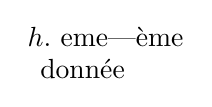
\begin{tikzpicture}[baseline=(given.base)]
\node[inner sep=0pt,anchor=base west] (given) at (0,0) {donnée};
\node[inner sep=0pt,anchor=base west] at (-0.16,0.40) {\inserted{$h$.\ \unsure{eme|ème}}};
\end{tikzpicture} de $1$. Les droites régulières $D$ ayant la propriété précédente (appelées ``droites cycliques'' par Kostant) sont conjuguées sous $W$, leur nombre est égal à $\operatorname{card}(W)/h$.
% The typed h. eme is interlinear, beginning slightly left of donnée; no caret establishes a linear insertion point.

NB Dans l'ensemble des droites cycliques, le groupe $(\underline{Z}/h\underline{Z})^{\handwritten{*}}$ opère\inserted{en commutant à l'action de $W$} librement; deux droites cycliques sont conjuguées sous l'action de ce groupe si et seulement si elles ont même stabilisateur dans $W$.
% archive sheet number: 2
